
Table \ref{tbl:results} shows the results of our systems with respect to the semantic evaluation metric of the CoNLL-08 shared task \citep{surdeanu08conll}. This metric not only measures the $F_1$ score in terms of the semantic arguments, but also includes the accuracy of the predicted predicate senses. %%Need more detailed explanation 
%The table also includes results from two existing approaches. The first one, Vicrey, was the winning system in the CoNLL 2008 shared task open track (here MALT parse trees were given). The second one, Johansson, won the closed track of the same competition (here parse trees had to be predicted, too). The results for their systems were taken from the overview paper~(cite) and only show the $F_1$ scores for the verbal/PropBank predicates.\footnote{Extracted from Table 16 of the mentioned paper.}

To put these results into context, let us compare them to those of the participants of the CoNLL 2008 shared task (see the last three rows of table \ref{tbl:results}). \footnote{Results of other systems were extracted from Table 16 of the shared task overview paper \citep{surdeanu08conll}.} Our best model, Bottom-up, would reach the highest $F_1$ WSJ score, and second highest Brown score, for the open track. Here the best-performing participant was \citet{vickrey08applying}. 

Table \ref{tbl:results} also shows the results of the best~\citep{johansson08dependency} and fourth best system~\citep{zhao08parsing} of the closed track. We note that we do significantly worse than \citet{johansson08dependency}, and roughly equivalent to \citet{zhao08parsing}; this places us on the fourth rank of 19 participants. However, note that all three systems above us, as well as  \citet{zhao08parsing}, use parsers with at least about 90\% (unlabelled) accuracy on the WSJ test set (Johansson's parser even has about 92\% unlabelled accuracy).\footnote{Since our parses use a different label set we could not compare labelled accuracy.} By contrast, with about 87\% unlabelled accuracy our parses are significantly worse.   

%It would reach the 4th highest score (for both WSJ and Brown) for the closed track, only beaten by systems that use 
%use highly optimized (ensemble-based, 2nd order, etc.) dependency parsers as input. In the closed track the highest score was obtain by \citet{johansson08dependency} system. Note that this comparison is based only on the results for verbal predicates.

\begin{table}[ht]
    \centering
    \begin{tabular}{|p{3.0cm}|c|c|c|}\hline
        System                    & Devel      & WSJ       & Brown \\\hline 
        Full                      & $76.93$  & $79.09$ & $67.64$ \\
%        Full (-arg)               &          &         &         \\
        Bottom-up                 & $77.96$  & $80.26$ & $67.75$ \\
        Bottom-up (-arg)          & $77.57$  & $79.37$ & $66.70$ \\
        Pipeline                  & $75.69$  & $78.19$ & $64.66$ \\
        \hline
        Vickrey                   &   N/A    & $79.75$ & $69.57$ \\
        Johansson                 &   N/A    & $86.37$ & $71.87$ \\
        Zhao                      &   N/A    & $79.40$ & $66.38$ \\
        \hline
    \end{tabular}
    \caption{Labelled $F_1$ scores of our five systems using CoNLL-08
    evaluation.} 
    %IV-
    %Systems that do not explicitely model the $isArgument$ decisions are marked with (-arg).}
    \label{tbl:results}
\end{table}

%% Unlabelled dependency accuracy for WSJ
% We (Charniak): 86.77%
% Johansson: 92.45
% che: 90.03
% ciaramita: 90.20
% zhao: 89.86 


\subsection{Joint Model vs. Pipeline}
Table \ref{tbl:results} suggests that by including sense disambiguation into the joint model (as is the case for all systems but the pipeline) significant improvements can be gained. Where do these improvements come from? We tried to answer this question by taking a closer look at how accurately the pipeline predicts the $isPredicate$, $isArgument$, $hasRole$, $role$ and $sense$ relations, and how this compares to the result of the joint bottom-up model.

Table \ref{tbl:predicates} shows that the joint model does significantly better (2\% points) when it comes to predicting the right roles and senses. This is particularly true for the case of the Brown corpus---here we gain about 10\% points for senses. These results suggest that the global formulae which assess the semantic frame of a predicate help in both ways: they can improve both senses and role labels simultanously. In contrast, the joint model does not help us to identify predicates and arguments; the score for all remaining hidden predicates remains roughly equal. 

The role labelling in figure \ref{fig:jointSense} illustrates how the joint model overcomes a limitation of the pipeline approach. Here the argument identification and classification stage of the pipeline has wrongly picked `You'' the A0 role and ``lawyer'' the A2 role of the predicate ``realize''. Because the role ``A2'' (``created from'') only appears in the  ``02'' (``create'') sense of ``realize'', the sense disambiguation stage wrongly selects the ``02'' instead of the corrent ``01'' (``come to know'') sense. In contrast, the joint bottom-up model knows that by simply dropping ``You'' as argument all together and changing the ``A2'' to an ``A0'' label, the sense ``01'' becomes a very suitable and consistent choice (even though the role labelling itself might be slightly less likely).

\begin{table}[ht]

    \centering
    \begin{tabular}{|c|c|c|c|c|}\hline
      & \multicolumn{2}{c|}{WSJ} & \multicolumn{2}{c|}{Brown}\\
                                  & Pipe.  &  B.u.   & Pipe.  &  B.u. \\\hline 
        \emph{isPredicate}        & $96.6$ & $96.5$ & $92.2$  & $92.5$\\
        \emph{isArgument}         & $90.3$ & $90.4$ & $85.9$ & $86.6$ \\
        \emph{hasRole}            & $88.0$ & $87.7$ & $83.6$ & $83.6$ \\
        \emph{role}               & $75.4$ & $77.5$ & $64.2$ & $66.2$ \\
        \emph{sense}              & $85.5$ & $89.5$ & $67.3$ & $77.5$ \\\hline
    \end{tabular}
    \caption{$F_1$ scores for Markov Logic predicates; Pipe. refers to the Pipeline system, B.u. to the Bottom-up system.}
    \label{tbl:predicates}
\end{table}

\begin{figure}
\begin{center}
    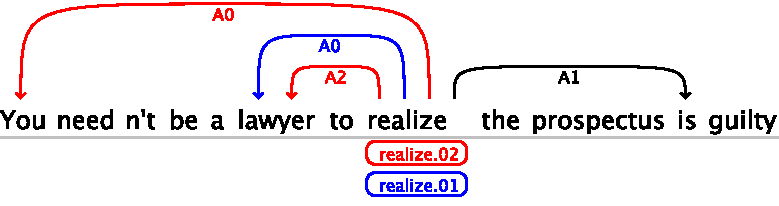
\includegraphics[scale=.58]{joint-sense-example}
\end{center}
\caption{Fragment of sentence in the development set that the pipeline model gets wrong: it picks the wrong sense (``02'') for ``realize'' and falsely assigns ``You'' the A0 role and ``lawyer'' the A2 role.}
\label{fig:jointSense}
\end{figure}


% I don't quite understand why we did isArg vs no isArg :-S. Maybe, too late to
% bring the issue. I just put two columns, if I put dev and brown, they get too
% big.
% SR: Huh? Without isArg we wouldn't need to jointly predict args for ALL predicates of one sentence. So this is to justify the joint model, and the fact that we explicitely model isArgument (different from all other SRL models I know). 

\subsection{Modelling if a Token is an Argument}
In table \ref{tbl:results} we also observe that improvements can be made if we explicitely model the decision whether a token is a semantic argument of some predicate or not. As we mentioned in section \ref{sec:model}, this aspect of our model requires us to jointly perform inference for all predicates of a sentence, and hence our results justify the per-sentence SRL approach proposed in this paper.

In order to analyse where these improvements come from, we again list our results on a per-SRL-predicate basis. Table \ref{tbl:isArg} shows that by including the $isArgument$ predicate and the corresponding formulae we gain around 0.6\% and 1.0\% points across the board for WSJ and Brown, respectively. As shown in table \ref{tbl:results}, these improvements result in about 1.0\% improvements for both WSJ and Brown in terms of the CoNLL 2008 metric. Hence, an explicit model of the ``is an argument'' decision helps the SRL at all levels. 

How the $isArgument$ helps to improve the overall role labelling score can be illustrated with the example in figure \ref{fig:isArg}. Here the model without a hidden $isArgument$ predicate fails to attach the preposition ``on'' to the predicate ``start.01'' (here 01 refers to the sense of the predicate). Apparently the model has not enough confidence to assign the preposition to either ``start.01'' or ``get.03'', so it just drops the argument altogether. However, because the $isArgument$ model knows that most prepositions have to be modifying some predicate, pressure is created that forces a decision between the two predicates. And because for the role model ``start.01'' looks like a better fit than ``get.03'', the correct attachment is found.

%%example
\begin{figure}
\begin{center}
    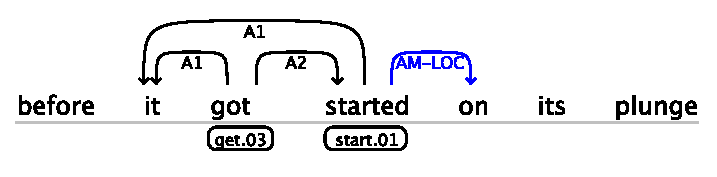
\includegraphics[scale=.62]{is-arg-example}
\end{center}
\caption{Sentence of the development for which the bottom-up model w/o $isArgument$ fails to attach the preposition ``on'' as a ``AM-LOC'' for ``started'' that complete bottom-up model attaches correctly.   }
\label{fig:isArg}
\end{figure}


\begin{table}[ht]

    \centering
    \begin{tabular}{|c|c|c|c|c|}\hline
      & \multicolumn{2}{c|}{WSJ} & \multicolumn{2}{c|}{Brown}\\
                                  & w/o     & w/     & w/o    & w/  \\\hline 
        \emph{isPredicate}        & $96.3$  & $96.5$ & $91.4$ & $92.5$\\
%%        \emph{isArgument}         &         & $86.6$ &        & $86.6$ \\
        \emph{hasRole}            & $87.1$  & $87.7$ & $82.5$ & $83.6$ \\
        \emph{role}               & $76.9$  & $77.5$ & $65.2$ & $66.2$ \\
        \emph{sense}              & $88.3$  & $89.0$ & $76.1$ & $77.5$ \\\hline
    \end{tabular}
    \caption{$F_1$ scores for Markov Logic predicates; w/o refers to a Bottom-up system without isArgument predicate, w/ refers to a Bottom-up system with isArgument predicate.}
    \label{tbl:isArg}
\end{table}

\subsection{Efficiency}
In the previous sections we have shown that our joint model indeed does better than an equivalent pipeline system. However, usually most joint approaches comes at a price: efficiency. Interestingly, in our case we observe the opposite: our joint model is actually faster than the pipeline. This can be seen in table \ref{tbl:nocpi}, where we list the time it took for several different system to process the WSJ and Brown test corpus, respectively. When we compare the times for the bottom-up model to those of the pipeline, we note that the joint model is twice as fast. While the invidual stages within the pipeline may be faster than the joint system (even when we sum up inference times), extracting results from one system and feeding them into another creates overhead which offsets this potential reduction.  

Table \ref{tbl:nocpi} also lists the runtime of a bottom-up system that solves the inference problem by fully grounding the Markov Network that the Markov Logic model describes, mapping this network to an Integer Linear Program, and finding the most likely assignment using an ILP solver. This system (Bottom-up (-CPI)) is four times slower than the equivalent system that uses Cutting Plane Inference  (Bottom-up). This suggests that if we were to implement the same joint model using ILP instead of Markov Logic, we either would be significantly slower, or we would need to implement a Cutting Plane algorithm for the corresponding ILP formulation---when we use Markov Logic this algorithm comes ``for free''. 
% \begin{table}[ht]

%     \centering
%     \begin{tabular}{|p{2.5cm}|c|c|c|}\hline
%         System                           & Training & Testing   & Testing \\
%                                          &          & WSJ       & Brown   \\\hline 
%         Full model                       & $5.1$h   & $9.2$m    & $1.5$m  \\
%         Bottom-up                        & $4.3$ih  & $9.5$m    & $1.6$m  \\
%         Full model w/o \emph{isArgument} &          &           &         \\
%         Bottom-up  w/o \emph{isArgument} & $3.9$h   & $12.5$m   & $1.5$m \\
%         Pipeline                         & $5.0$h   & $18.9$m   & $2.9$m \\\hline
%     \end{tabular}
%     \caption{Testing and training times for the systems.}
%     \label{tbl:times}
% \end{table}

\begin{table}[ht]

    \centering
    \begin{tabular}{|p{3.0cm}|c|c|}\hline
        System                           & WSJ       & Brown   \\\hline 
        Full                             & $9.2$m    & $1.5$m  \\
        Full (-CPI)                      & $38.4$m   & $7.47$m  \\
        Bottom-up                        & $9.5$m    & $1.6$m  \\
        Bottom-up (-CPI)                 & $38.8$m   & $6.9$m  \\
        Pipeline                         & $18.9$m   & $2.9$m  \\\hline
    \end{tabular}
    \caption{Testing times for full model and bottom-up when CPI algorithm is
    not used.}
    \label{tbl:nocpi}
\end{table}


%7. Results
%7.1 Joint/Bottom-up vs pipeline
%- Illustrate that we get dramatic improvements in sense
%disambiguation, but not in other parts. Stress effect on Brown
%- Show table that compares isPredicate & role & frameLabel results for
%pipeline vs joint models (this would show that no gain in isPredicate
%and role, but in frameLabel)
%- Give example from dev-set
%7.2 With isArg vs without isArg
%- illustrate that we get improvements in all sections
%- show table that compares individual predicate scores (dev, wsj,
%brown) for isArg vs w/o isArg
%- maybe find example?
%7.3 (Maybe) Full vs Bottom-up again (maybe not because in other paper)
%7.4 Efficiency
%- Illustrate that training the model jointly comes at no extra cost
%(we can train as fast/faster with the joint bottom up model than with
%a pipeline)
%- Illustrate that inference is much more efficient when compared to an
%equivalent ILP-only system (which is basically the w/o CPI system)
%- Can we also have a sentence/second column for testing?
%
%
%Pipeline
%**************
%         isPredicate    : 0.958,0.959,0.958,0.959,0.959
%          isArgument    : 0.890,0.892,0.891,0.891,0.891
%            hasLabel    : 0.870,0.873,0.872,0.872,0.872
%                role    : 0.706,0.718,0.720,0.722,0.723
%          frameLabel    : 0.834,0.842,0.841,0.841,0.841
%
%         isPredicate    : 0.966,0.922
%          isArgument    : 0.903,0.859
%            hasLabel    : 0.880,0.836
%                role    : 0.754,0.642
%          frameLabel    : 0.855,0.673
%
%Times :
%trainning (hrs):
%stage1= 0.76
%stage2= 3.42
%stage3= 0.84
%total = 5.02
%testing:
%stage1: 5.44m, 42.68s
%stage2: 7.56m, 1.27m 
%stage3: 5.96m, 54.03s
%total: 18.96,  2.90m
%
%
%WSJ
%  Labeled precision:          (10284 + 4521) / (13021 + 5321) * 100 = 80.72 %
%  Labeled recall:             (10284 + 4521) / (14269 + 5260) * 100 = 75.81 %
%  Labeled F1:                 78.19
%
%Brown
%  Labeled precision:          (1335 + 555) / (1986 + 846) * 100 = 66.74 %
%  Labeled recall:             (1335 + 555) / (2210 + 804) * 100 = 62.71 %
%  Labeled F1:                 64.66
%
%
%
%Full model
%**************
%         isPredicate    : 0.958,0.959,0.958,0.958,0.958
%          isArgument    : 0.894,0.895,0.895,0.895,0.895
%            hasLabel    : 0.865,0.868,0.869,0.869,0.869
%                role    : 0.703,0.713,0.720,0.724,0.727
%          frameLabel    : 0.870,0.874,0.878,0.877,0.878
%
%         isPredicate    : 0.965,0.923
%          isArgument    : 0.906,0.869
%            hasLabel    : 0.879,0.838
%                role    : 0.755,0.646
%          frameLabel    : 0.885,0.771
%
%Times:
%Training :5.09 hrs
%Testing:
%WSJ          9.15m 
%Brown        1.58m 
%
%
%WSJ
%  Labeled precision:          (10423 + 4664) / (13348 + 5273) * 100 = 81.02 %
%  Labeled recall:             (10423 + 4664) / (14269 + 5260) * 100 = 77.25 %
%  Labeled F1:                 79.09
%
%Brown
%  Labeled precision:          (1369 + 621) / (2063 + 807) * 100 = 69.34 %
%  Labeled recall:             (1369 + 621) / (2210 + 804) * 100 = 66.03 %
%  Labeled F1:                 67.64
%
%
%Full model w/o isArg (NOTE: not with new formula2/ we need it with bottom-up model as well)
%**************
%
%       isPredicate      : 0.955,0.955,0.954,0.955,0.955
%            hasLabel    : 0.860,0.863,0.866,0.865,0.865
%                role    : 0.710,0.722,0.727,0.730,0.730
%          frameLabel    : 0.869,0.874,0.875,0.876,0.875
%
%         isPredicate    : 0.963,0.910
%            hasLabel    : 0.872,0.818
%                role    : 0.752,0.638
%          frameLabel    : 0.878,0.761
%
%Times (hrs)
%Training: 4.58
%Testing:
%WSJ       9.53m 
%Brown     1.43m 
%
%
%
%WSJ
%  Labeled precision:          (10308 + 4615) / (13132 + 5257) * 100 = 81.15 %
%  Labeled recall:             (10308 + 4615) / (14269 + 5260) * 100 = 76.41 %
%  Labeled F1:                 78.71
%
%Brown
%  Labeled precision:          (1324 + 609) / (1973 + 797) * 100 = 69.78 %
%  Labeled recall:             (1324 + 609) / (2210 + 804) * 100 = 64.13 %
%  Labeled F1:                 66.84
%
%
%
%Bottom up
%**************
%         isPredicate    : 0.958,0.960,0.960,0.960,0.959
%          isArgument    : 0.893,0.895,0.895,0.894,0.894
%            hasLabel    : 0.867,0.870,0.869,0.870,0.869
%                role    : 0.728,0.738,0.743,0.746,0.747
%          frameLabel    : 0.872,0.878,0.885,0.887,0.883
%
%         isPredicate    : 0.965,0.925
%          isArgument    : 0.904,0.866
%            hasLabel    : 0.877,0.836
%                role    : 0.775,0.662
%          frameLabel    : 0.890,0.775
%
%Times:
%Training 4.26 hrs
%Testing:
%WSJ          9.53m 
%Brown        1.55m 
%
%WSJ
%  Labeled precision:          (10315 + 4590) / (12349 + 5262) * 100 = 84.63 %
%  Labeled recall:             (10315 + 4590) / (14269 + 5260) * 100 = 76.32 %
%  Labeled F1:                 80.26
%
%Brown
%  Labeled precision:          (1327 + 591) / (1836 + 812) * 100 = 72.43 %
%  Labeled recall:             (1327 + 591) / (2210 + 804) * 100 = 63.64 %
%  Labeled F1:                 67.75
%
%
%NO CPI 
%**************
%         isPredicate    : 0.959,0.958,0.958,0.957,0.957
%          isArgument    : 0.894,0.896,0.895,0.895,0.893
%            hasLabel    : 0.867,0.869,0.870,0.868,0.867
%                role    : 0.708,0.720,0.726,0.727,0.727
%          frameLabel    : 0.873,0.878,0.880,0.879,0.879
%
%         isPredicate    : 0.964,0.925
%          isArgument    : 0.905,0.865
%            hasLabel    : 0.877,0.836
%                role    : 0.775,0.661
%          frameLabel    : 0.886,0.778
%
%Times:
%training: 6.51 hrs
%testing:
% WSJ        38.06m
% Brown       6.73m 
%
%WSJ     
%  Labeled precision:          (10323 + 4546) / (12384 + 5267) * 100 = 84.24 %
%  Labeled recall:             (10323 + 4546) / (14269 + 5260) * 100 = 76.14 %
%  Labeled F1:                 79.98
%
%Brown
%  Labeled precision:          (1324 + 600) / (1833 + 812) * 100 = 72.74 %
%  Labeled recall:             (1324 + 600) / (2210 + 804) * 100 = 63.84 %
%  Labeled F1:                 68.00
%
%
%Without linguistic
%**************
%
%
%
%
%bottom-up w/o isArg
%**************
%         isPredicate    : 0.953,0.955,0.955,0.955,0.954
%            hasLabel    : 0.859,0.863,0.863,0.863,0.862
%                role    : 0.725,0.739,0.742,0.743,0.745
%          frameLabel    : 0.870,0.875,0.877,0.876,0.876
%
%         isPredicate    : 0.963,0.914
%            hasLabel    : 0.871,0.825
%                role    : 0.769,0.652
%          frameLabel    : 0.883,0.761
%
%Times
%Training: 3.84 hrs
%Testing:
%WSJ         12.52m
%Brown        1.50m 
%
%WSJ
%  SEMANTIC SCORES:
%  Labeled precision:          (10218 + 4495) / (12293 + 5252) * 100 = 83.86 %
%  Labeled recall:             (10218 + 4495) / (14269 + 5260) * 100 = 75.34 %
%  Labeled F1:                 79.37
%
%
%Brown
%  Labeled precision:          (1298 + 578) / (1806 + 805) * 100 = 71.85 %
%  Labeled recall:             (1298 + 578) / (2210 + 804) * 100 = 62.24 %
%  Labeled F1:                 66.70
%
%


